\documentclass[a4paper, oneside]{memoir}
\usepackage[utf8]{inputenc}
\usepackage[T1]{fontenc}
\usepackage{pifont}
\usepackage{amssymb}
\usepackage{fourier}
\usepackage[dvipsnames]{xcolor}
\usepackage{tikz}
\usepackage{pdfpages}
\usepackage[sfdefault]{roboto}
\usepackage{color}

% Styles
\tikzstyle{teamshare} = [below, text width=5.4cm, inner sep = 0.5cm, text=white, align=center]
\tikzstyle{cardtext} = [below, text width=5.9cm, inner sep = 0.25cm, text centered]
\setlrmarginsandblock{0.9cm}{*}{1}
\setulmarginsandblock{1.2cm}{*}{1}
\checkandfixthelayout[nearest]
\pagestyle{empty}

% Define Commands
\newcommand{\condition}[1]{\textbf{#1}}
\newcommand{\character}[1]{\textbf{#1}}
\newdimen\titlespacing
\titlespacing=0.15cm

% Define Seperators
\newcommand{\seperator}[1]{\\ \vspace{\titlespacing} \hrulefill {} \tiny \bfseries #1 \normalfont \normalsize \hrulefill \\ \vspace{\titlespacing}}
\newcommand{\seperatoraction}{\seperator{POWER}}
\newcommand{\seperatordescription}{\seperator{DESCRIPTION}}
\newcommand{\seperatorcondition}{\seperator{CONDITION}}
\newcommand{\seperatorwin}{\seperator{HOW TO WIN}}
\newcommand{\redwinsection}{
	\seperatorwin
	You win if \character{Harry Potter} does not gain the \condition{dead} condition due to \character{Voldemort}.
}
\newcommand{\greenwinsection}{
	\seperatorwin
	\small You win if \character{Harry Potter} gains the \condition{dead} condition due to the \character{Voldemort}.
}
\newcommand{\titlefrom}[1]{\\ \tiny > from #1 <\normalsize}

% Begin Document
\begin{document}
\noindent 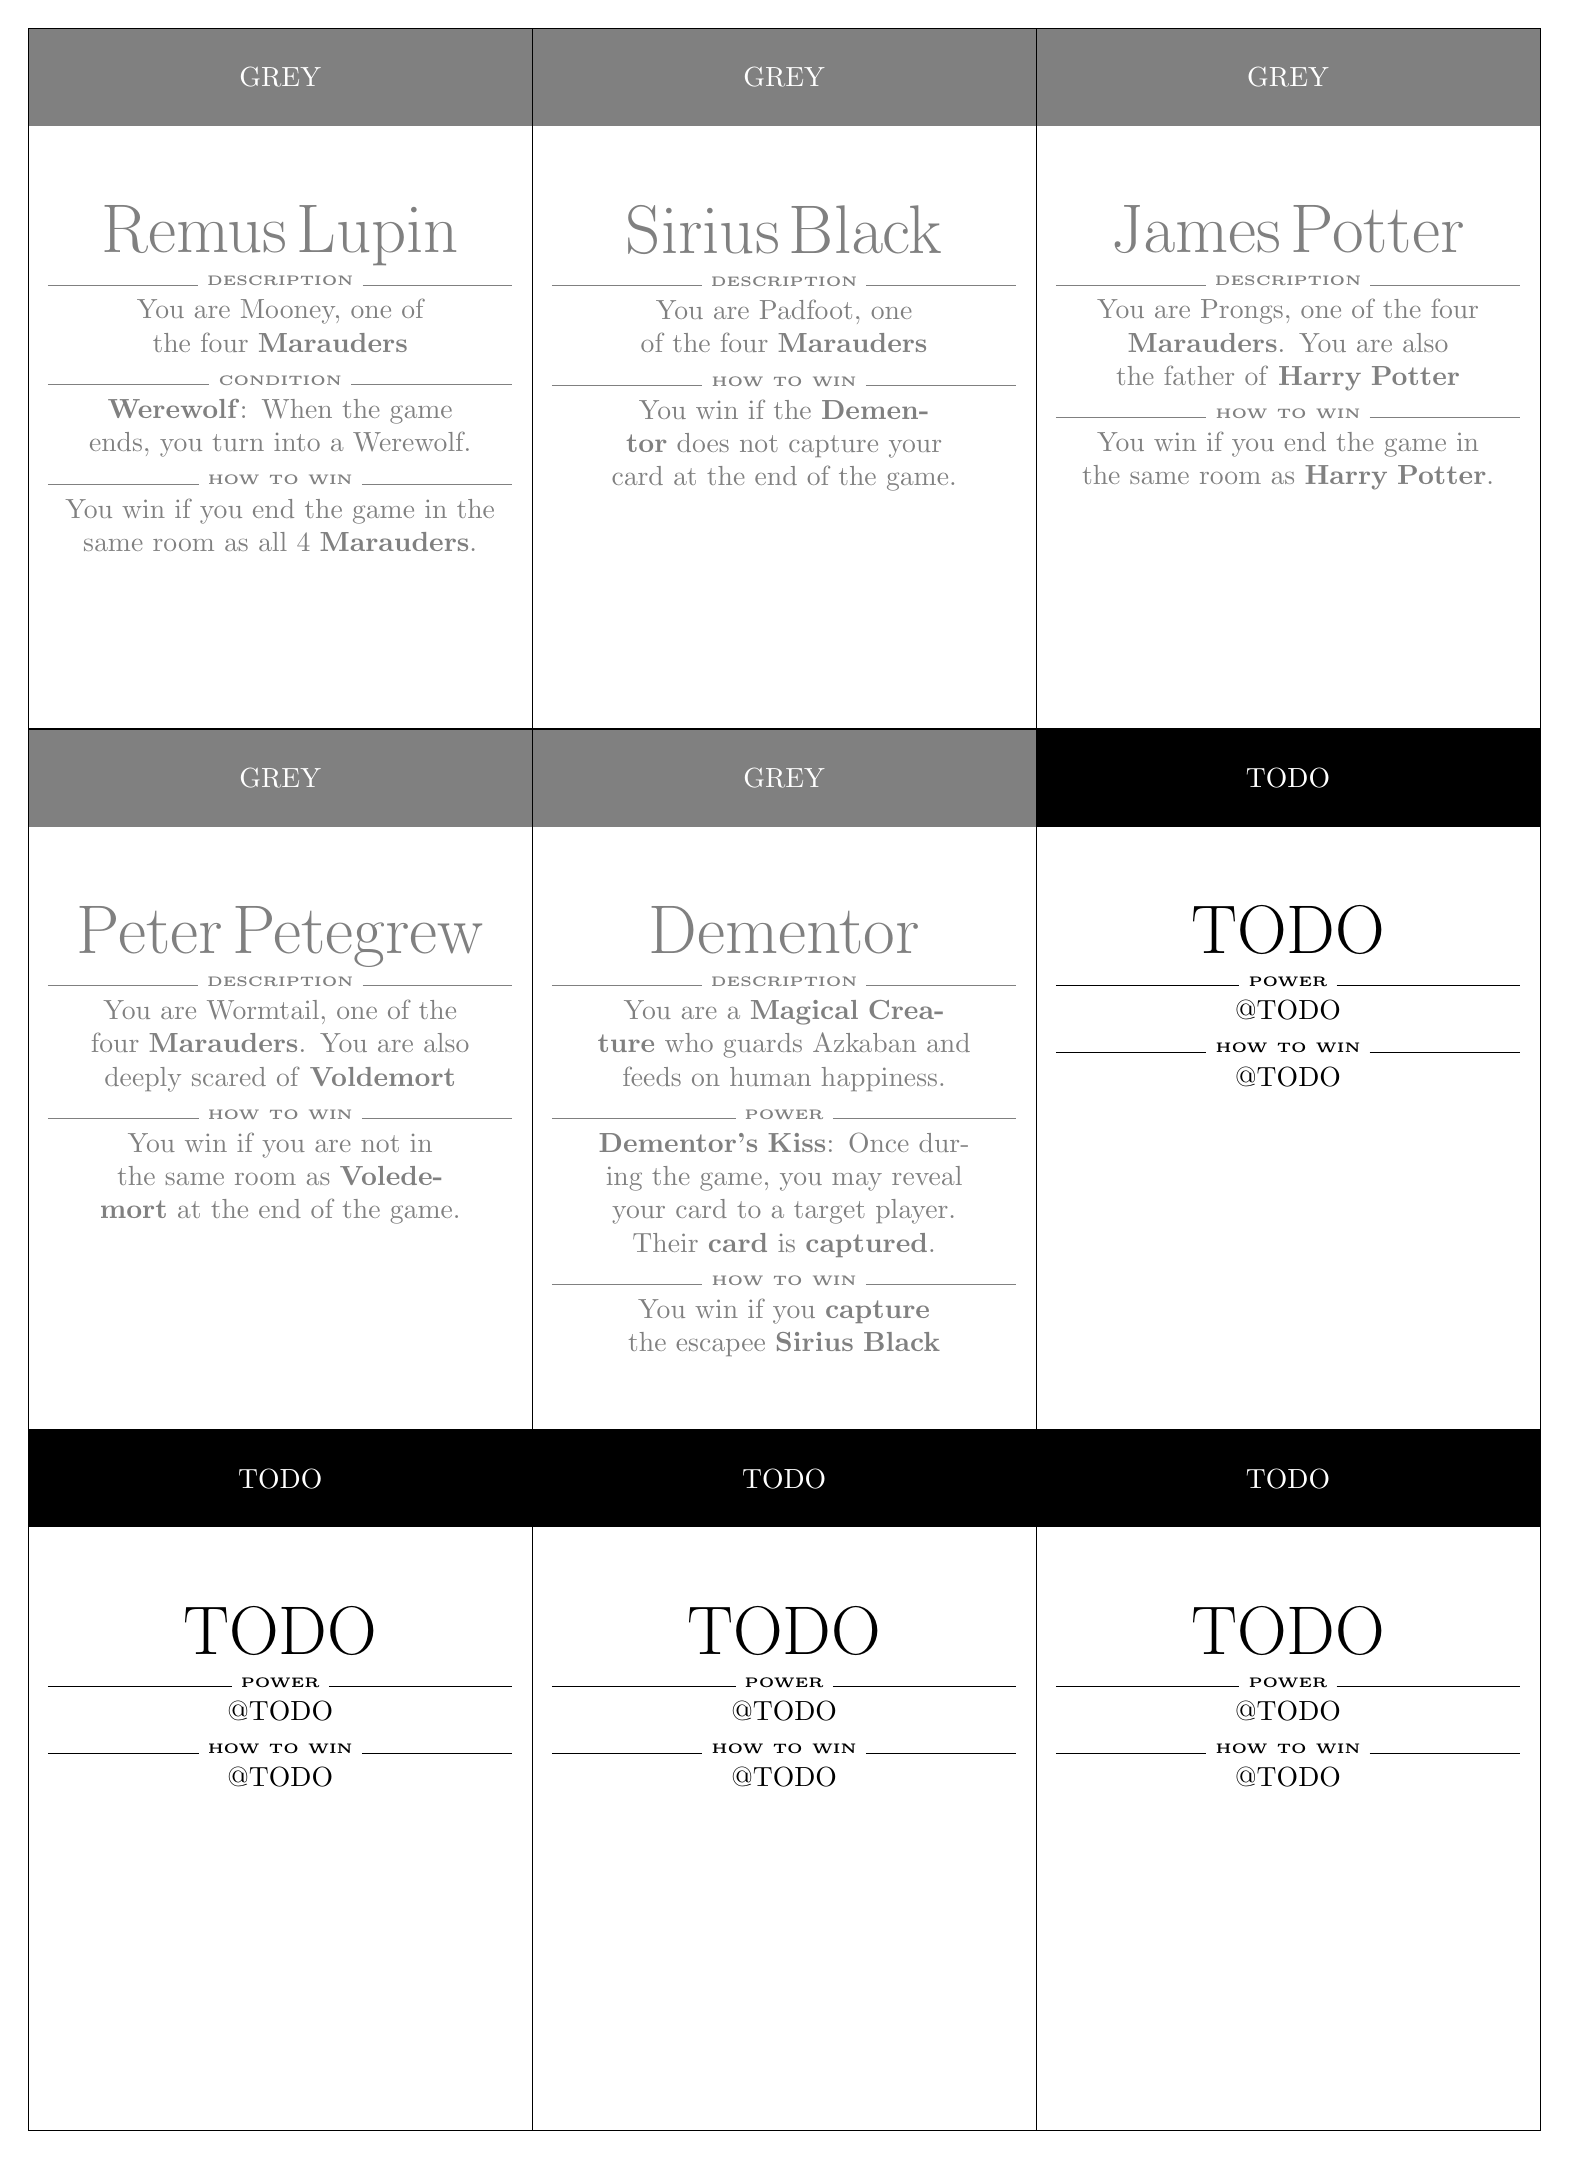
\begin{tikzpicture}[outer sep=0]

	% PROFESSOR LUPIN
	\node[teamshare, fill=gray] (1) at (3.2,26.7) {\HUGE GREY};
	\node[cardtext, text=gray] at (3.2,24.7) {
		{\Huge Remus Lupin}
		\seperatordescription
		You are Mooney, one of the four \condition{Marauders}
		\seperatorcondition
		\condition{Werewolf}: When the game ends, you turn into a Werewolf.
		\seperatorwin
		You win if you end the game in the same room as all 4 \condition{Marauders}.
	};
	
	% SIRIUS BLACK
	\node[teamshare, fill=gray] at (9.6,26.7) {\HUGE GREY};
	\node[cardtext, text=gray] at (9.6,24.7) {
		{\Huge Sirius Black}
		\seperatordescription
		You are Padfoot, one of the four \condition{Marauders}
		\seperatorwin
		You win if the \character{Dementor} does not capture your card at the end of the game.
	};
	
	% JAMES POTTER
	\node[teamshare, fill=gray] at (16,26.7) {\HUGE GREY};
	\node[cardtext, text=gray] at (16,24.7) {
		{\Huge James Potter}
		\seperatordescription
		You are Prongs, one of the four \condition{Marauders}. You are also the father of \character{Harry Potter}
		\seperatorwin
		You win if you end the game in the same room as \character{Harry Potter}.
	};
	
	% PETER PETTEGREW
	\node[teamshare, fill=gray] at (3.2,17.8) {\HUGE GREY};
	\node[cardtext, text=gray] at (3.2,15.8) {
		{\Huge Peter Petegrew}
		\seperatordescription
		You are Wormtail, one of the four \condition{Marauders}. You are also deeply scared of \character{Voldemort}
		\seperatorwin
		You win if you are not in the same room as \character{Voledemort} at the end of the game.
	};
	
	% DEMENTOR
	\node[teamshare, fill=gray] at (9.6,17.8) {\HUGE GREY};
	\node[cardtext, text=gray] at (9.6,15.8) {
		{\Huge Dementor}
		\seperatordescription
		You are a \condition{Magical Creature} who guards Azkaban and feeds on human happiness.
		\seperatoraction
		\condition{Dementor's Kiss}: Once during the game, you may reveal your card to a target player. Their \character{card} is \character{captured}.
		\seperatorwin
		You win if you \character{capture} the escapee \character{Sirius Black}
	};
	
	% TODO
	\node[teamshare, fill=black] at (16,17.8) {\HUGE TODO};
	\node[cardtext, text=black] at (16,15.8) {
		{\Huge TODO}
		\seperatoraction
		@TODO
		\seperatorwin
		@TODO
	};
	
	% TODO
	\node[teamshare, fill=black] at (3.2,8.9) {\HUGE TODO};
	\node[cardtext, text=black] at (3.2,6.9) {
		{\Huge TODO}
		\seperatoraction
		@TODO
		\seperatorwin
		@TODO
	};
	
	% TODO
	\node[teamshare, fill=black] at (9.6,8.9) {\HUGE TODO};
	\node[cardtext, text=black] at (9.6,6.9) {
		{\Huge TODO}
		\seperatoraction
		@TODO
		\seperatorwin
		@TODO
	};
	
	% TODO
	\node[teamshare, fill=black] at (16,8.9) {\HUGE TODO};
	\node[cardtext, text=black] at (16,6.9) {
		{\Huge TODO}
		\seperatoraction
		@TODO
		\seperatorwin
		@TODO
	};
	
	\draw (0,0) -- (19.2,0);
	\draw (0,8.9) -- (19.2,8.9);
	\draw (0,17.8) -- (19.2,17.8);
	\draw (0,26.7) -- (19.2,26.7);
	\draw (0,0) -- (0,26.7);
	\draw (6.4,0) -- (6.4,26.7);
	\draw (12.8,0) -- (12.8,26.7);
	\draw (19.2,0) -- (19.2,26.7);

\end{tikzpicture}
\includepdf[pages={1}, angle=0]{cardsbackground.pdf}
\end{document}